\section{Background}
Understanding the impact cell resolution ($dx$) has on model behavior, delta morphology, dynamics, and stratigraphy is important, as model resolution influences the model's runtime (Chapter \ref{chap:resruntime}).

\section{Model Runs}
A set of 4 cell resolution values are used and model runs are conducted in triplicate.
These runs are at ``field-scale" using parameters similar to those from previous studies \cite{Liang2016, Liang2016a}.
The YAML below provides information about the parameter set used.\\

\noindent \texttt{YAML} configuration file: \vspace{-6pt}
\begin{boxedverbatim}
ensemble: 3
Length: 7500
Width: 15000
timesteps: 5000
L0_meters: 150.0
N0_meters: 300.0
SLR: 36e-10  # slight maybe 3 mm/yr SLR
save_dt: 300000  # every 10 timesteps (dt = 30000)

matrix:
  dx:
    - 30.0
    - 50.0
    - 75.0
    - 100.0
\end{boxedverbatim}

\section{Results}
Final topographies, as well as corresponding channel maps are visualized (Figures \ref{fig:res_finaltopo} \& \ref{fig:res_chanmap}).
Channel fraction timeseries for all runs is computed (Figure \ref{fig:res_chanfrac_timeseries}), as is the channelized fraction over the final 50 years for each run for which box-plots for each cell resolution are created (Figure \ref{fig:res_chanfrac}).
Channel widths and depths are calculated along azimuthal transects based on the location of surface channels (from Figure \ref{fig:res_chanmap}), using the final topography (from Figure \ref{fig:res_finaltopo}), the average width and depth values are plotted (Figure \ref{fig:res_depth_v_width}), as are the width-to-depth ratios as a function of model cell resolution (Figure \ref{fig:res_wd}).

\begin{figure}[!ht]
	\makebox[\textwidth][c]{
	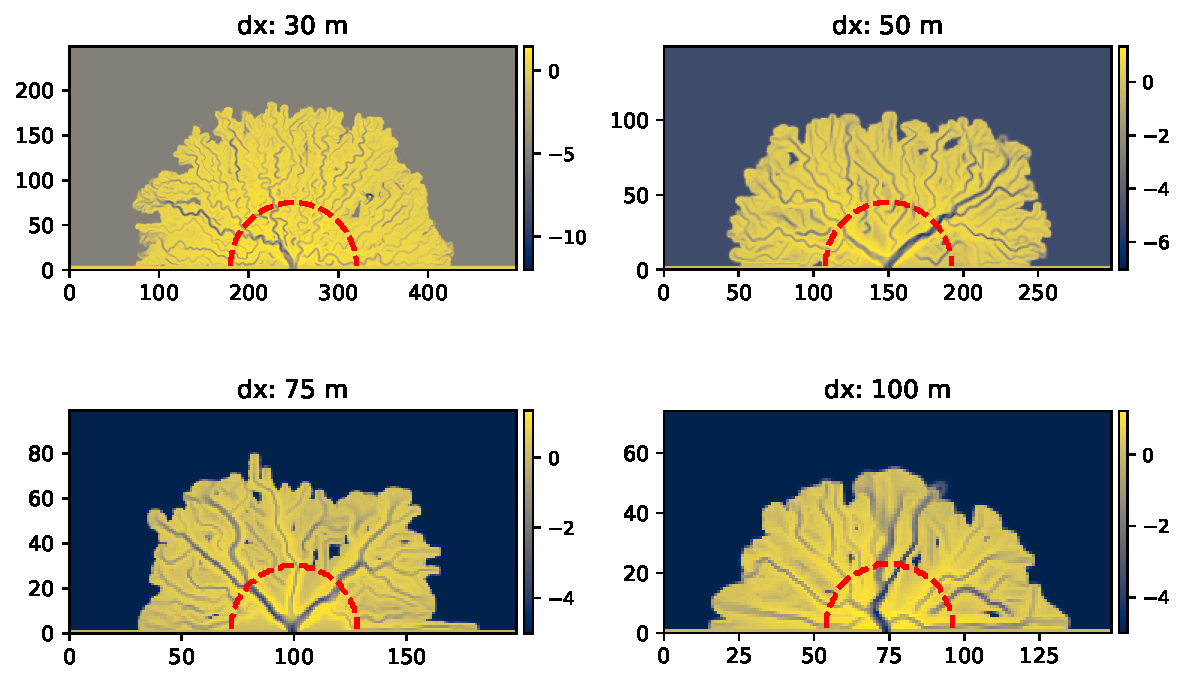
\includegraphics[width=\textwidth]{CellResAnalysis/figs/circ_planview.pdf}
	}	
	\caption{Final topography for different cell resolutions with the location of the azimuthal transect used for channel width and depth measurements shown as a dashed red line.}
	\label{fig:res_finaltopo}
\end{figure}

\begin{figure}[!ht]
	\makebox[\textwidth][c]{
	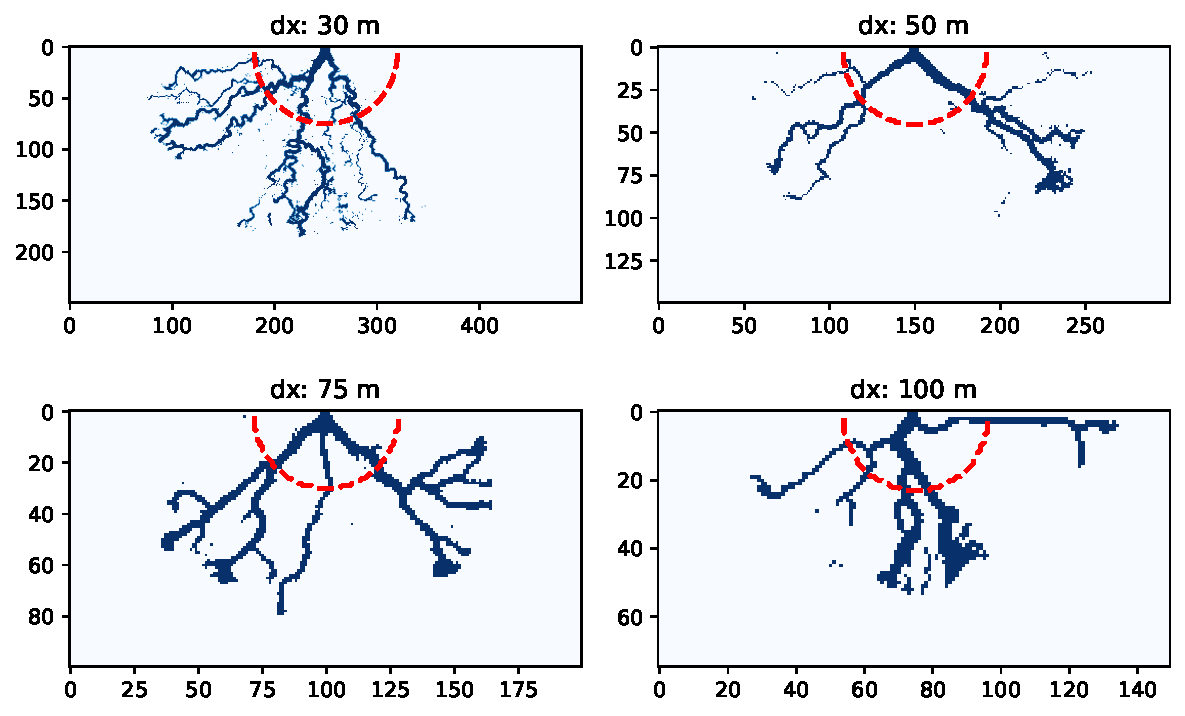
\includegraphics[width=\textwidth]{CellResAnalysis/figs/circular_planview.pdf}
	}	
	\caption{Binary surface channel maps at the final timestep for the different cell resolutions, surface channels identified as cells with water velocities exceeding 0.3 m/s.}
	\label{fig:res_chanmap}
\end{figure}

\begin{figure}[!ht]
	\makebox[\textwidth][c]{
	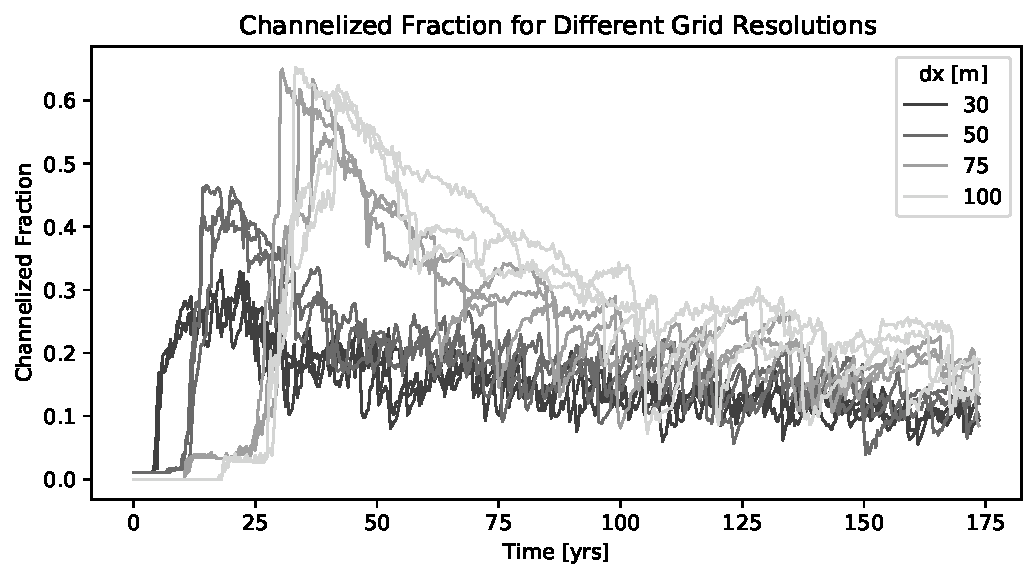
\includegraphics[width=\textwidth]{CellResAnalysis/figs/chanfrac_timeseries.pdf}
	}	
	\caption{Timeseries of channelized fraction values for all of the model runs.}
	\label{fig:res_chanfrac_timeseries}
\end{figure}

\begin{figure}[!ht]
	\makebox[\textwidth][c]{
	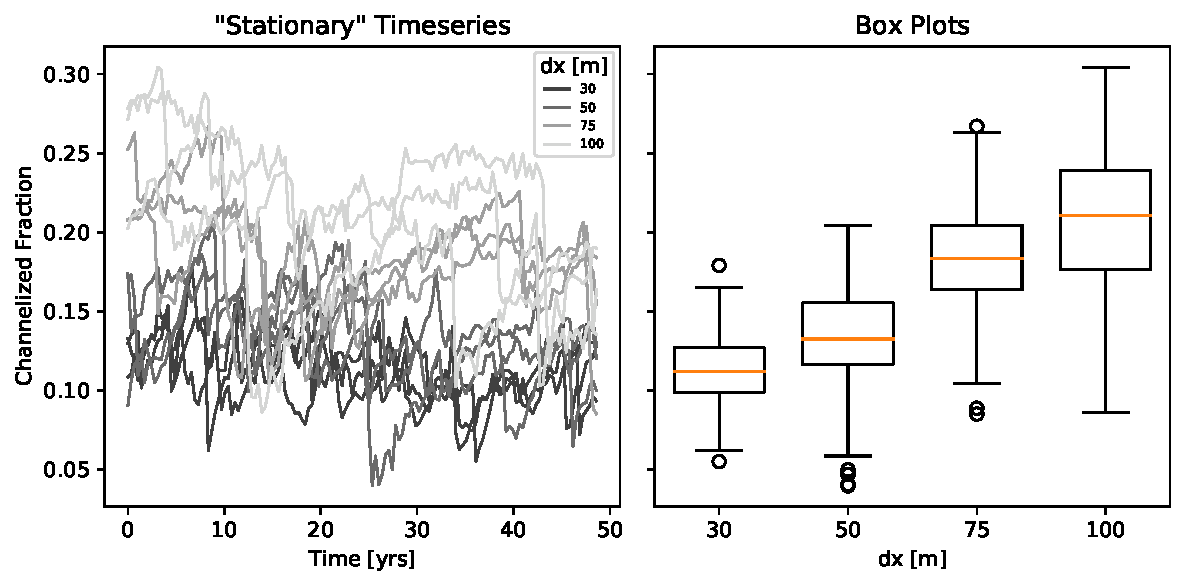
\includegraphics[width=\textwidth]{CellResAnalysis/figs/chanfrac_stationary.pdf}
	}	
	\caption{Channelized fraction values for the final 50 years of each simulation (Left), and box plots of those values for each cell resolution tested (Right).}
	\label{fig:res_chanfrac}
\end{figure}

\begin{figure}[!ht]
	\makebox[\textwidth][c]{
	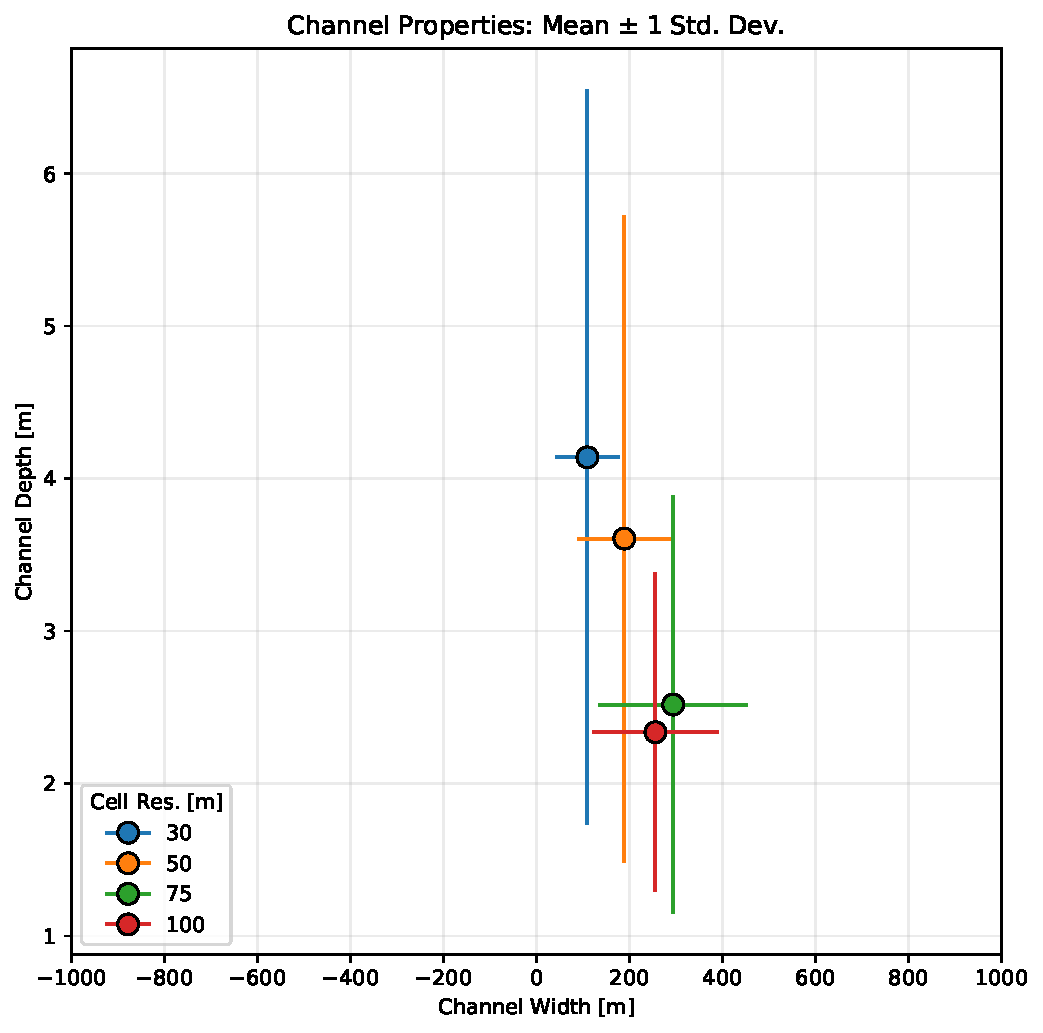
\includegraphics[width=\textwidth]{CellResAnalysis/figs/depth_v_width.pdf}
	}	
	\caption{Plots of average channel depth vs average channel width values as calculated along the azimuthal transects.}
	\label{fig:res_depth_v_width}
\end{figure}

\begin{figure}[!ht]
	\makebox[\textwidth][c]{
	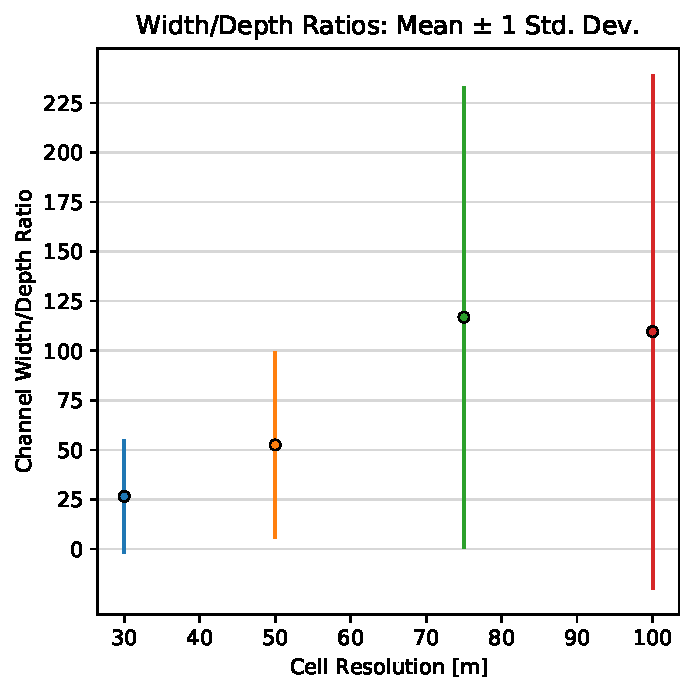
\includegraphics[width=\textwidth]{CellResAnalysis/figs/widthdepth_ratio.pdf}
	}	
	\caption{Width-to-depth ratios of the surface channels as a function of model cell resolution.}
	\label{fig:res_wd}
\end{figure}

\section{Conclusions}
Model cell resolution does not only impact the time it takes to run the model, surface properties are impacted as well.
As the model grid resolution becomes more coarse, channel width-to-depth ratios increase as the channels are forced to widths which are multiples of the grid resolution, although the input conditions are unchanged.
The fraction of the surface that is channelized increases as the model becomes more coarse for a similar reason.
It is therefore important to think about the resolution of the cells when designing a pyDeltaRCM model run; for larger deltas it may be acceptable to move to a coarser cell resolution, but for small ``Wax Lake-like" deltas, it is probably not advisable to move to cells any larger than 50m.

\clearpage
\bibliographystyle{plainnat}
\bibliography{bib/bib}